\chapter{绪论} \label{chapter:intro}

\section{引言}

\section{地球与人类,是否无独有偶?}

由古至今,人类在宇宙中的所处的位置就一直魂牵梦绕着人们的思绪。这个难题既
包括了人类居住的地球在空间上是否独特,另一方面也包含了人类(或生命)在宇
宙中的唯一性与否。正因人类拥有了可思考问题的大脑,因而在这个问题上的观测
与探索也从未曾停歇。

首先,行星科学(Planetology)是一门古老的以观测为基础的科学。早在公元前,古
希腊等各大文明已有天文学家(如伊巴谷)统计了相当可观的夜空发光天体的运行与
方位。而在以托勒密为代表所提倡的地心说主导了这个星球一千多年后,文艺复兴时
期的哥白尼等人通过观测提出了日心说。自此地球在空间位置谜团便开始层层被揭开,
地球的面貌也愈发完善地展现在了人类的面前。


\begin{figure}[ht]
\centering
\begin{subfigure}[b]{.45\textwidth}
\centering
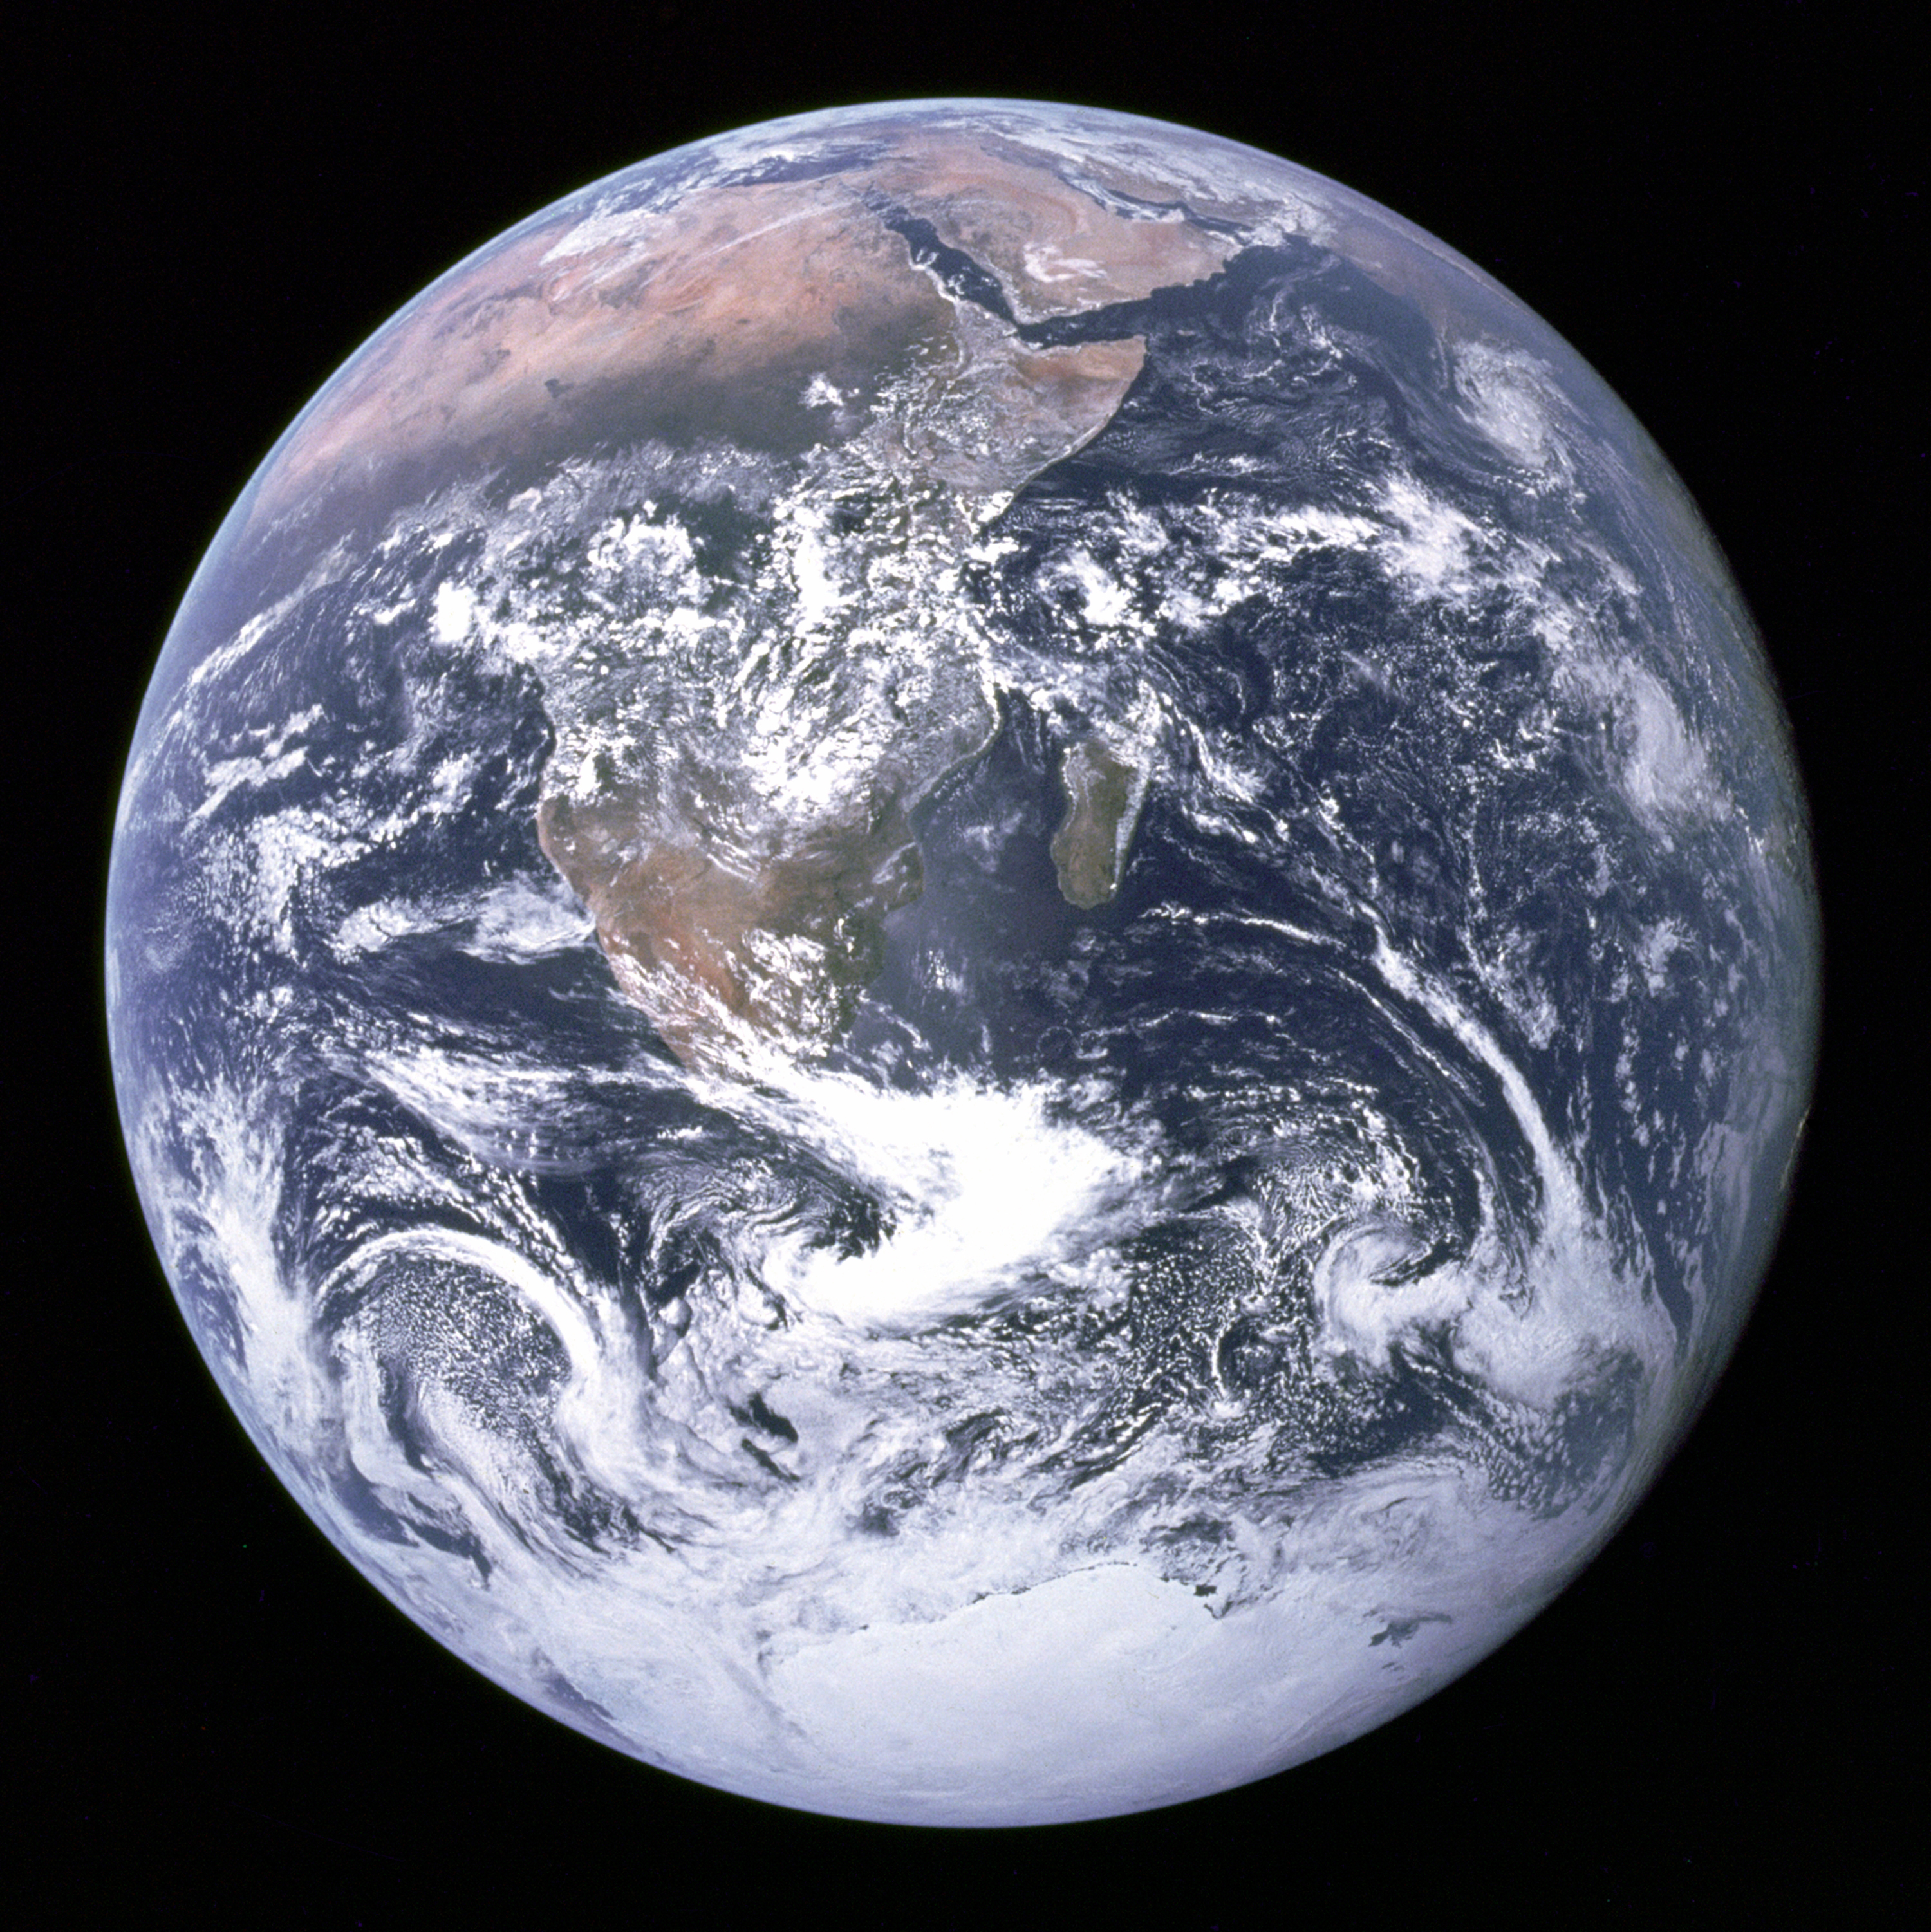
\includegraphics[width=0.95\textwidth]{figures/fig1a_Apollo17_BlueMarble.jpg}
\caption{subcaption 1}
\label{fig:sub1}
\end{subfigure}
\begin{subfigure}[b]{.45\textwidth}
\centering
\includegraphics[width=0.95\textwidth]{figures/fig1b_Horizon_PaleBlueDot.jpg}
\caption{subcaption 2}
\label{fig:sub2}
\end{subfigure}
\caption{Caption}
\label{fig:fig} 
\end{figure}


以往人们通过哲学方法来思考生命的唯

史前古希腊哲学家通过观测认为


太阳系内行星与地球的运动规律之探求,


到被称作现代天文之父的哥白尼所描述的日心说
体系,






从史前古希腊哲学家对太
阳系内行星与地球运动规律的探求

人类拥有双眼和思考

仰望星空

人类是独一无二的吗? Bruno


\section{系外行星的定义}

行星定义是什么?

在英文上 exoplanet 与 extrasolar planet 则是完全不同的词性来源。


\subsection{系外行星扼要史}

行星科学(Planetology)是一门古老的以观测为基础的科学:从史前古希腊哲学家对太
阳系内行星与地球的运动规律之探求,到被称作现代天文之父的哥白尼所描述的日心说
体系,人类从诞生之始就默默地注视着这些夜空的「神行者」。而作为专注于研究太阳
系以外的行星系统(简称:系外行星)科学,研究对象则跳脱出传统可观测的太阳系各
大行星,转向了银河系内其它恒星的周围。

探测到第一颗类太阳恒星周围的行星 51 Peg b 

\subsection{探测手段}

\subsection{行星形成理论}



